\section{Methodology}
\label{section:interview-methods}

This section describes the methods for selecting, conducting, and analying the interviews.
First, I describe the analytical approach. Then I discuss the method for selecting interviews
and provide an anonymized summary of the participants. Lastly, I share a table that summarizes
the themes that came out of the interviews and which sections discuss each theme.


\subsection{Thematic Analysis}
This section describes a multiple-case study using interviews with energy
planners, decision makers, and community advocates at local and state levels.
The interviewees were chosen to exemplify maximum variation cases
\cite{flyvbjerg_five_2006}. The participants and cases in this study vary in
perspective and context in order to create a holistic narrative about energy
planning within Illinois. A multiple-case study also enhances validity by
enabling replication and comparison \cite{johannsen_designing_2021,
yin_case_2018}. Further, since one purpose of this study is to evaluate the
design and applicability of the tool, \ac{osier}, a multiple-case study design
will strengthen software changes and feature additions, and support \ac{osier}'s
use in other locations and contexts. The raw data include interview
transcriptions and the relevant municipal climate and energy plans, if
available. The interviews were transcribed with the ``listen and revise'' method
using the Whisper transcription tool \cite{battaglia_listen_2024}. This method has two steps. 
First, I transcribe the interview using Whisper. Second, I listen back to the interview and
revise the transcription to correct errors. Whisper uses
\ac{ai} to automate the transcription process. Both the data and the \ac{ai}
model used to transcribe the interview audio were hosted locally (i.e., without
an internet connection), eliminating privacy concerns
\cite{battaglia_listen_2024}. Figure \ref{fig:whisper} shows a screenshot of the
Whisper interface. 

\begin{figure}[htbp!]
    \centering
    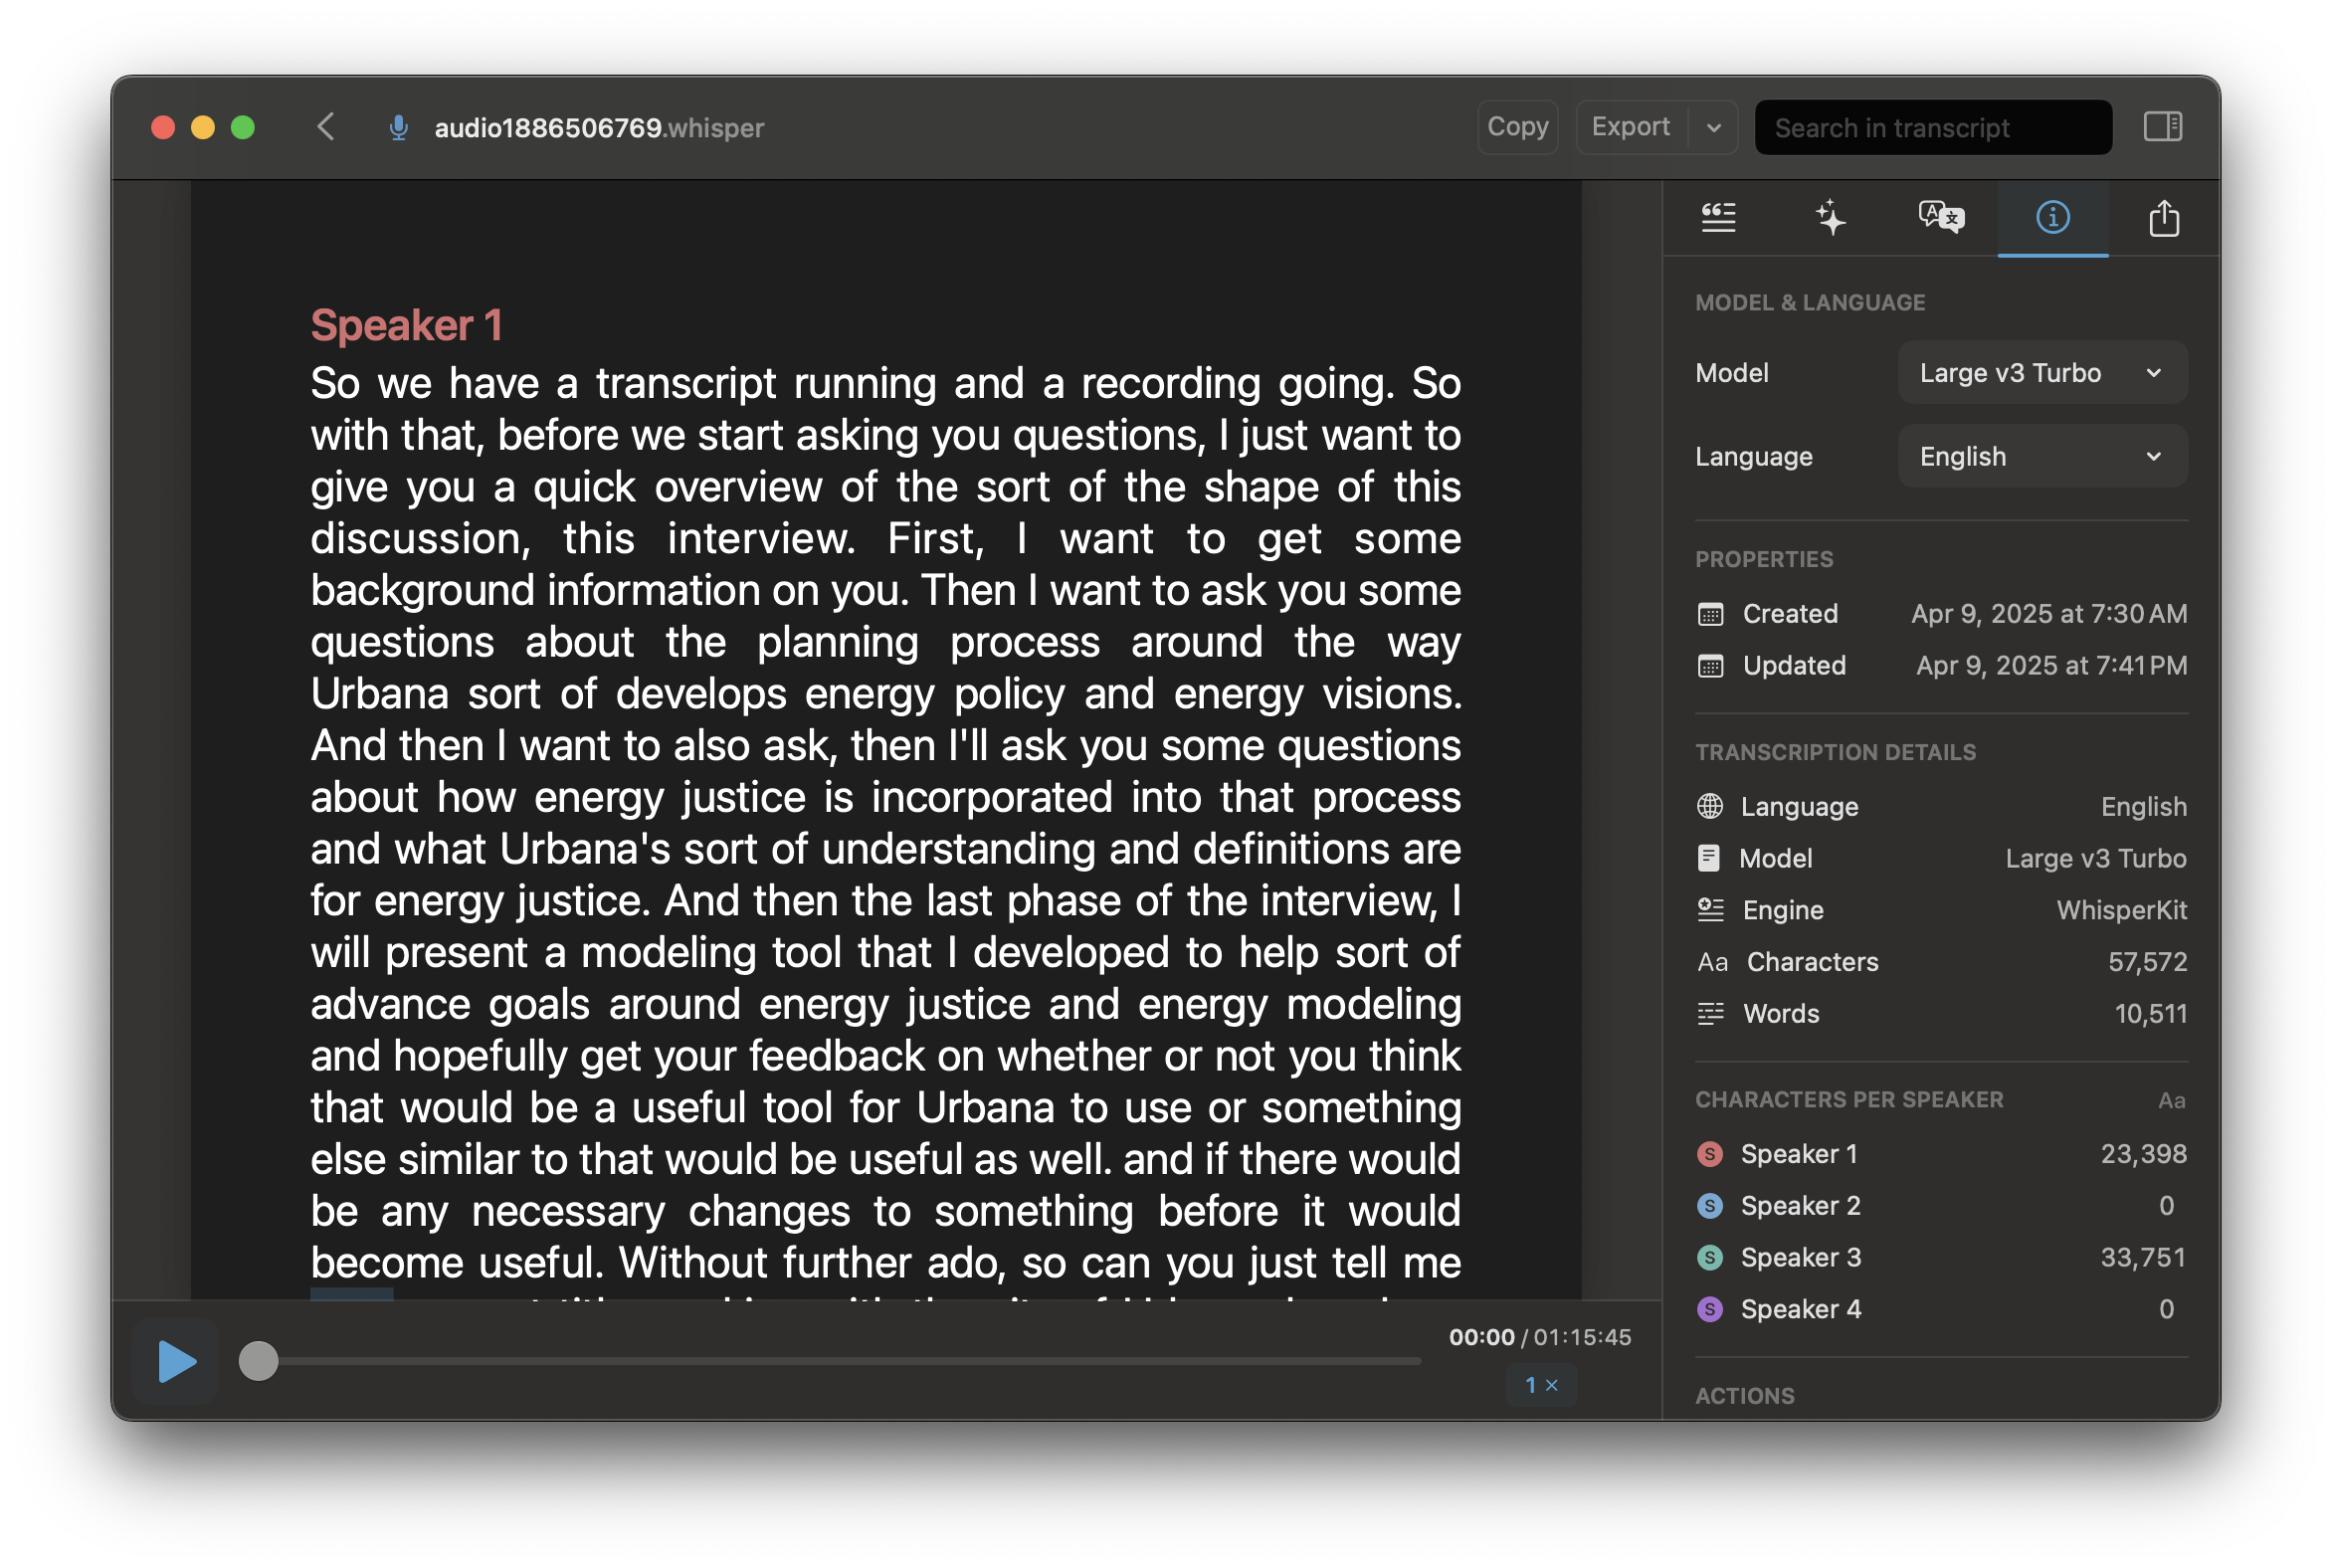
\includegraphics[width=0.8\columnwidth]{figures/07_interview_chapter/whisper-screenshot.png}
    \caption{A screenshot of an interview transcribed with Whisper. To protect
    the privacy of the interviewees, only ``Speaker 1'' is shown. ``Speaker 1''
    is the author of this thesis.}
    \label{fig:whisper}
\end{figure}

The transcribed interviews were initially coded using a deductive approach that involves a
predefined set of codes. These initial codes aligned with the three aims of this study:
\begin{enumerate}
    \item identify how (if) energy models are used to support energy planning at
    local and state levels,
    \item determine the ways energy justice or equity are incorporated into
    planning decisions
    \item assess the usefulness of a new modeling tool, \ac{osier}.
\end{enumerate} 
However, I combined this with an inductive process to develop additional codes.
The benefits of this hybrid strategy are that it allows comparing and
contrasting the results of the present study with existing literature and
producing insights novel to this study. The interview coding step was also
performed locally with the \texttt{Taguette} tool \cite{rampin_taguette_2021}.
Figure \ref{fig:taguette} shows a screenshot of the \texttt{Taguette} software.

\begin{figure}[htbp!]
    \centering
    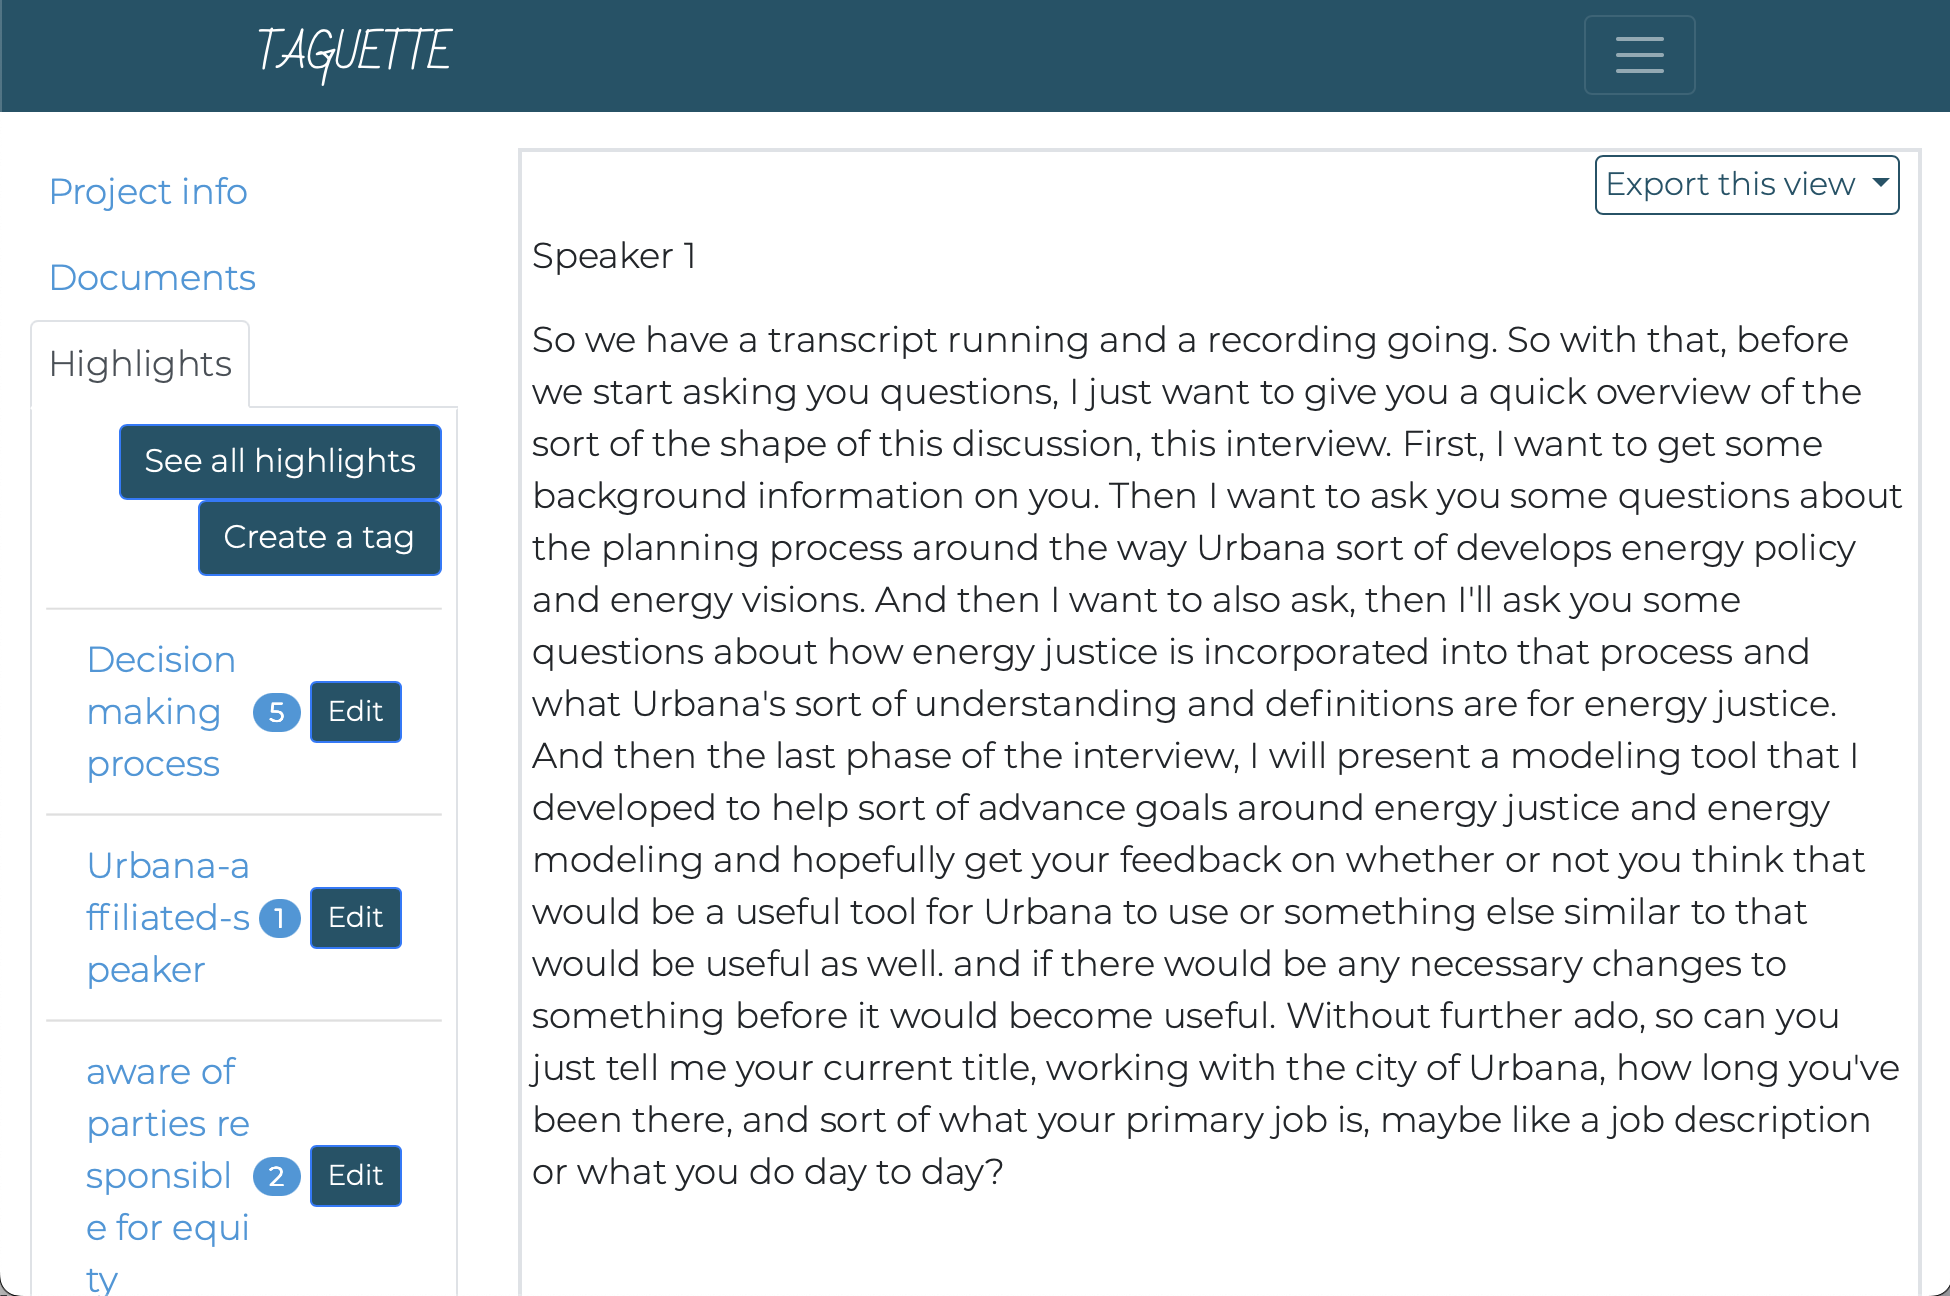
\includegraphics[width=0.8\columnwidth]{figures/07_interview_chapter/taguette-screenshot}
    \caption{A screenshot of the interview transcribed in Figure \ref{fig:whisper}
    loaded into \texttt{Taguette} for initial coding.}
    \label{fig:taguette}
\end{figure}

\subsection{Interview Data Collection}

A total of thirteen interviews were conducted virtually using the Zoom
teleconferencing software through the second half of 2024 and beginning of 2025,
using a semi-structured approach based on an interview guide designed according
to five main topics (for details, see Appendix \ref{chapter:interview-guide}).
\begin{enumerate}
    \item Background --- learn about the interviewees' experience and background
    with energy planning in their context.
    \item Existing planning processes --- clarify the processes used to develop
    climate action plans and energy policies.
    \item Conceptions of justice or equity --- elucidate the extent to which
    justice informs energy policies and plans.
    \item Use of models in planning processes --- identify if energy models are
    used and overall perceptions of modeling.
    \item Assessment of the \ac{osier} tool --- introduce \ac{osier} through a
    short presentation and invite reactions and feedback from the interviewee.
\end{enumerate}
The interviewees were chosen through a combination of
purposive\footnote{Purposive sampling selects participants based on specific
characteristics or expertise \cite{ahmed_how_2024}.} and snowball
\footnote{Snowball sampling involves participants referring others that also
match the research criteria \cite{ahmed_how_2024}. In this case, interviewees
connected me with other energy planners in their network.} sampling to identify
staff with sufficient and relevant energy planning experience. Each interviewee
is involved in decision-making, planning, or advocacy in their respective
context. Table \ref{tab:interviewees} summarizes the interviewees for this
study. The \textit{organization} column refers to the organization that either
employs, or is represented by, the interviewee. The \textit{type} column assigns
the interviewee to a broad category including:
\begin{enumerate}
    \item practitioner --- someone involved in the process of energy planning
    and/or carries out policy directives from policymakers,
    \item advocate --- a person or organization that lobbies for policy outcomes
    on behalf of a group of stakeholders,
    \item policymaker --- someone who participates in the ultimate
    decision-making related to energy policy.
\end{enumerate}
    
\begin{table}[ht!]
    \centering
    \caption{Interview participant codes and summary}
    \label{tab:interviewees}
    \begin{tabular}{llll}
        \toprule
        Number & Participant Code & Organization & Type \\
        \midrule
        1& UP1 &Urbana& Practitioner\\ % 
        2& UP2 &Urbana/\ac{uiuc}& Practitioner\\ % 
        3& UM1 &Urbana & Policy maker\\ % 
        4& UI1 & \ac{uiuc} & Practitioner\\ % 
        5& CP1 & Champaign & Practitioner\\ % 
        6& IP1 & \ac{icc} & Practitioner\\ % 
        8& IP2 & \ac{icc} & Practitioner\\ % JA
        7& IP3 & \ac{ipa} & Practitioner\\ % 
        9& IA1 &\ac{icea}& Advocate\\ % 
        10& IA2 &Illinois \ac{cub} & Advocate\\ % 
        11& NP1 & Naperville & Practitioner\\ % 
        12& NA1 &\acs{nest}&Advocate\\ % 
        13& NA2 &\acs{nest}&Advocate\\ % 
        \bottomrule
    \end{tabular}
\end{table}